\documentclass[11pt,a4paper]{report}
\usepackage[textwidth=37em,vmargin=30mm]{geometry}
\usepackage{calc,xunicode,amsmath,amssymb,paralist,enumitem,tabu,booktabs,datetime2,xeCJK,xeCJKfntef,listings}
\usepackage{tocloft,fancyhdr,tcolorbox,xcolor,graphicx,eso-pic,xltxtra,xelatexemoji}

\newcommand{\envyear}[0]{2025}
\newcommand{\envdatestr}[0]{2025-02-23}
\newcommand{\envfinaldir}[0]{webdb/2025/20250223/final}

\usepackage[hidelinks]{hyperref}
\hypersetup{
    colorlinks=false,
    pdfpagemode=FullScreen,
    pdftitle={Web Digest - \envdatestr}
}

\setlength{\cftbeforechapskip}{10pt}
\renewcommand{\cftchapfont}{\rmfamily\bfseries\large\raggedright}
\setlength{\cftbeforesecskip}{2pt}
\renewcommand{\cftsecfont}{\sffamily\small\raggedright}

\setdefaultleftmargin{2em}{2em}{1em}{1em}{1em}{1em}

\usepackage{xeCJK,xeCJKfntef}
\xeCJKsetup{PunctStyle=plain,RubberPunctSkip=false,CJKglue=\strut\hskip 0pt plus 0.1em minus 0.05em,CJKecglue=\strut\hskip 0.22em plus 0.2em}
\XeTeXlinebreaklocale "zh"
\XeTeXlinebreakskip = 0pt


\setmainfont{Brygada 1918}
\setromanfont{Brygada 1918}
\setsansfont{IBM Plex Sans}
\setmonofont{JetBrains Mono NL}
\setCJKmainfont{Noto Serif CJK SC}
\setCJKromanfont{Noto Serif CJK SC}
\setCJKsansfont{Noto Sans CJK SC}
\setCJKmonofont{Noto Sans CJK SC}

\setlength{\parindent}{0pt}
\setlength{\parskip}{8pt}
\linespread{1.15}

\lstset{
	basicstyle=\ttfamily\footnotesize,
	numbersep=5pt,
	backgroundcolor=\color{black!5},
	showspaces=false,
	showstringspaces=false,
	showtabs=false,
	tabsize=2,
	captionpos=b,
	breaklines=true,
	breakatwhitespace=true,
	breakautoindent=true,
	linewidth=\textwidth
}






\newcommand{\coverpic}[2]{
    % argv: itemurl, authorname
    Cover photo by #2~~(\href{#1}{#1})
}
\newcommand{\makeheader}[0]{
    \begin{titlepage}
        % \newgeometry{hmargin=15mm,tmargin=21mm,bmargin=12mm}
        \begin{center}
            
            \rmfamily\scshape
            \fontspec{BaskervilleF}
            \fontspec{Old Standard}
            \fontsize{59pt}{70pt}\selectfont
            WEB\hfill DIGEST
            
            \vfill
            % \vskip 30pt
            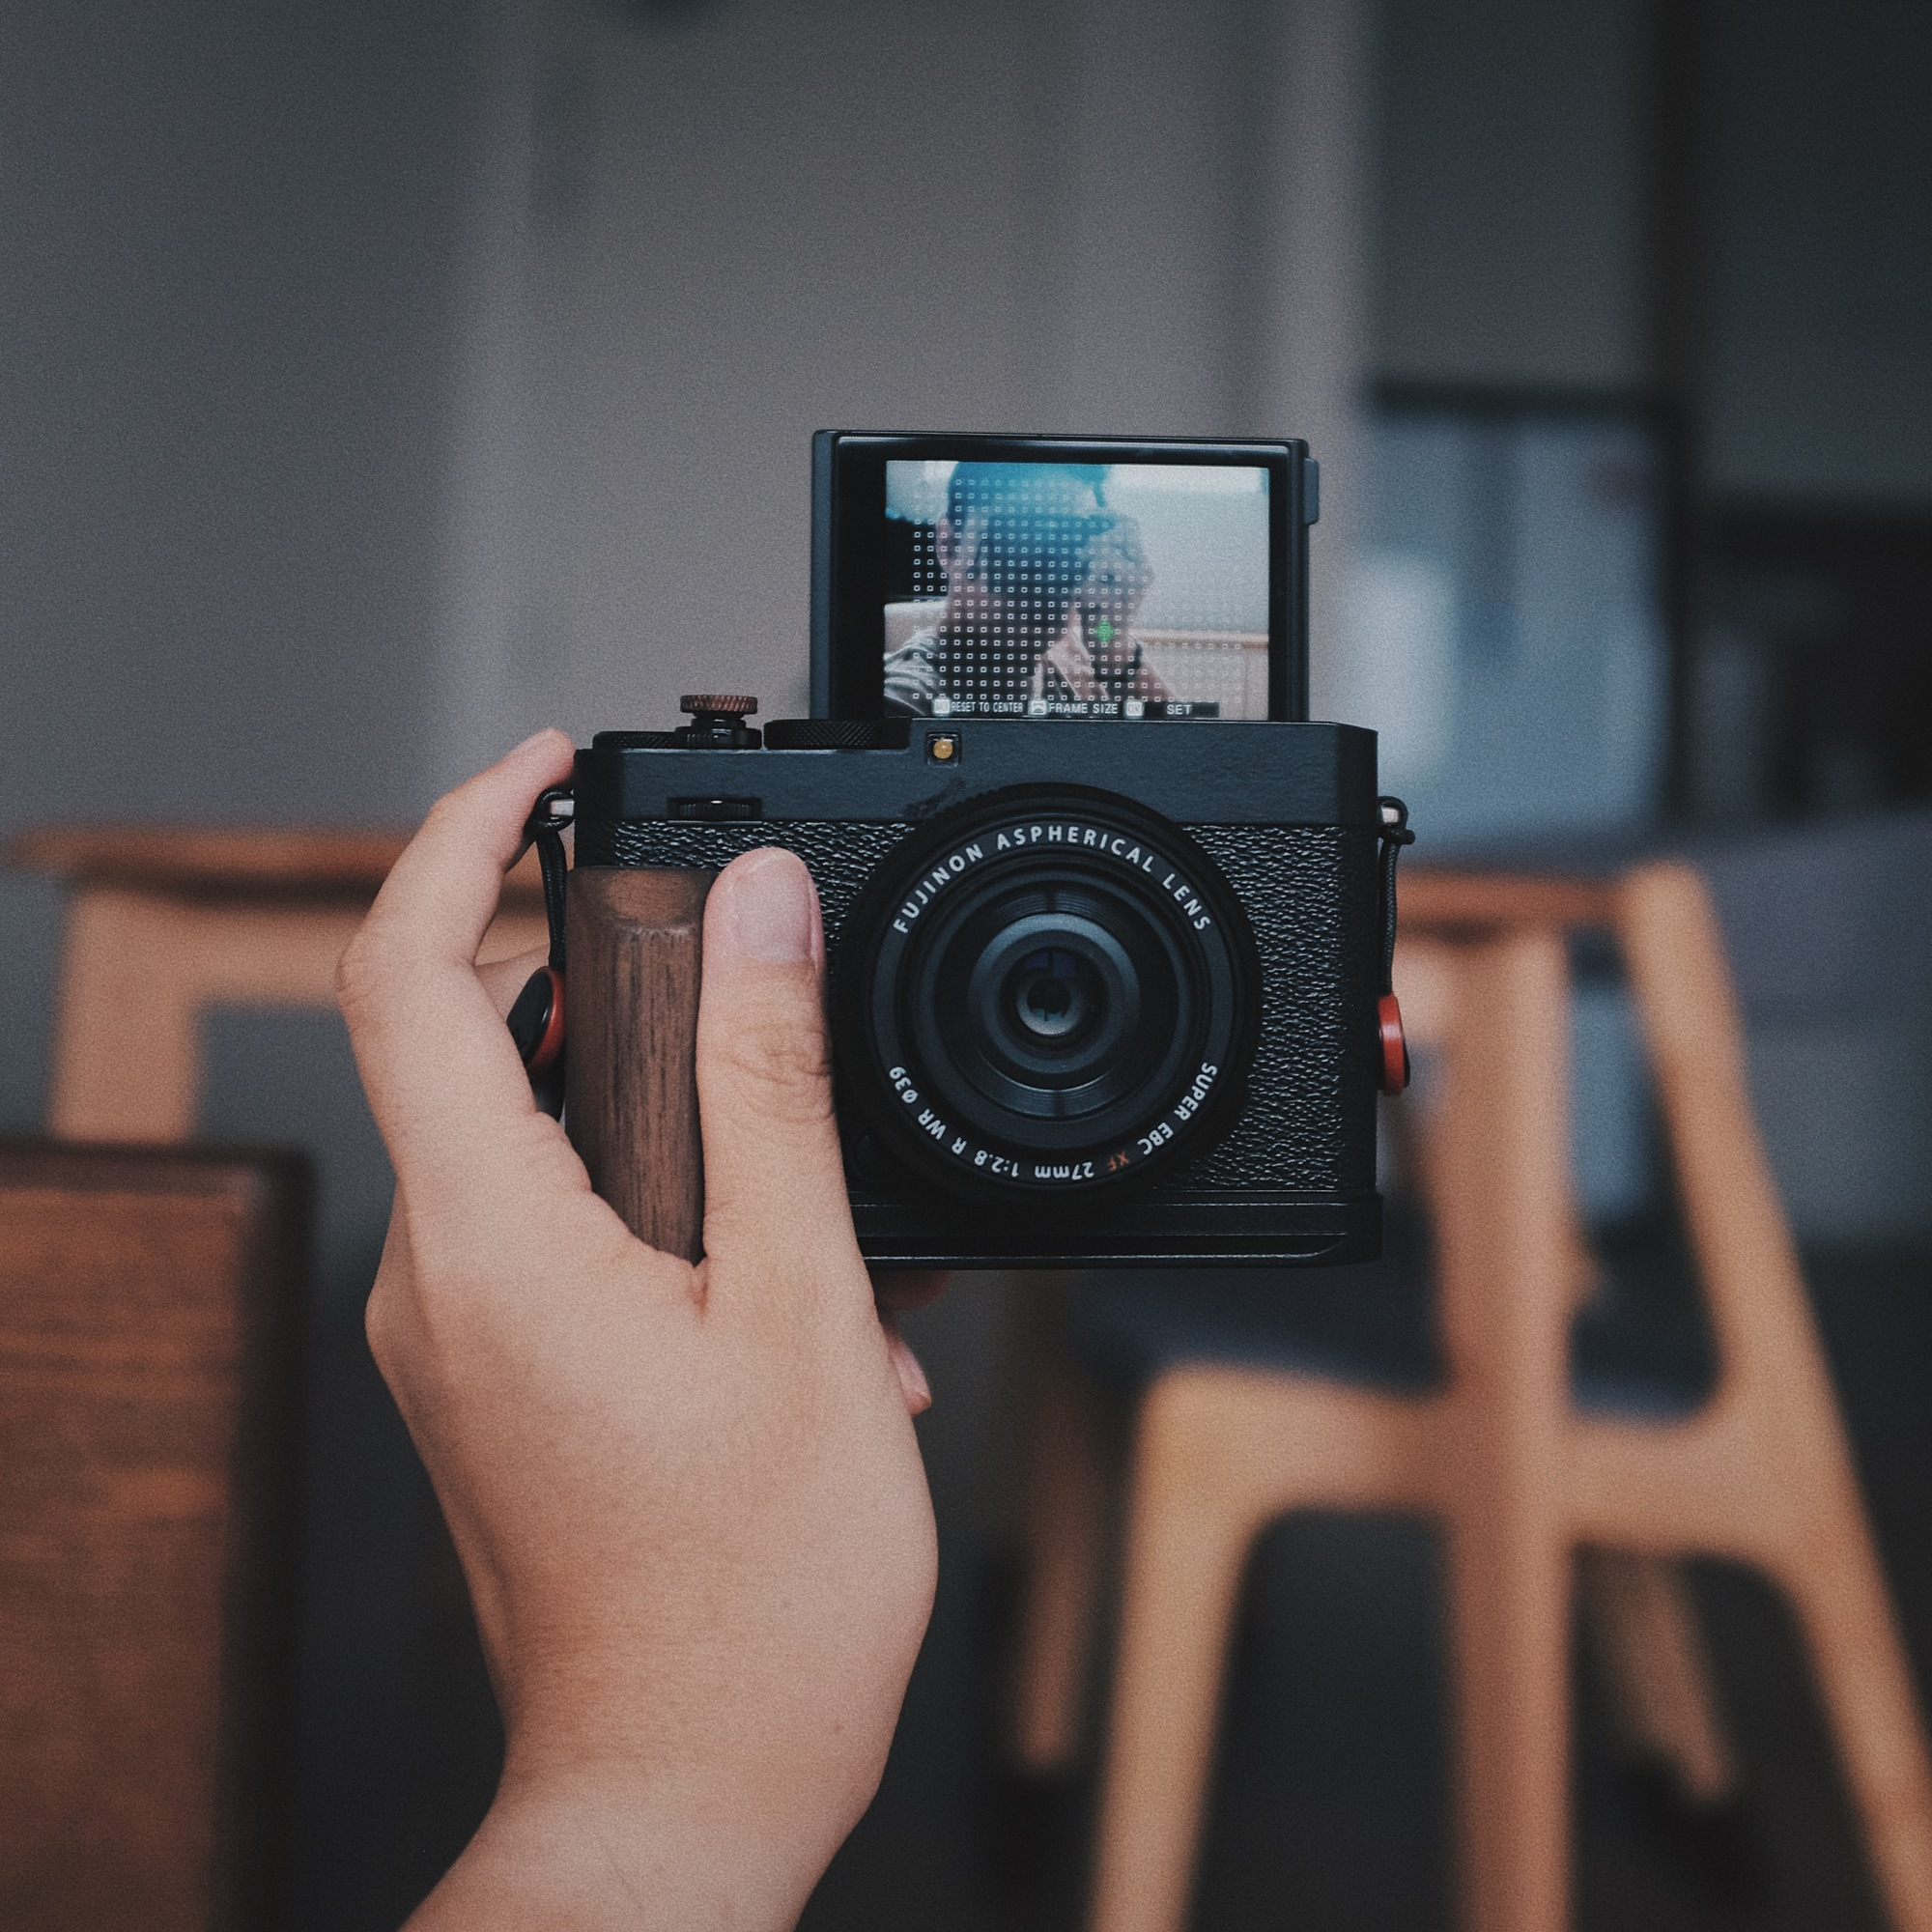
\includegraphics[width=\linewidth]{\envfinaldir/coverpic-prod.jpg}\par
            % \vskip 30pt
            \vfill

            \normalsize\rmfamily\scshape
            \copyright{} The Web Digest Project \hfill\large \envdatestr
        \end{center}
    \end{titlepage}
    % \restoregeometry
}
\newcommand{\simplehref}[1]{%
    \textcolor{blue!80!green}{\href{#1}{#1}}%
}
\renewcommand{\contentsname}{\center\Huge\sffamily\bfseries Contents\par\vskip 20pt}
\newcounter{ipartcounter}
\setcounter{ipartcounter}{0}
\newcommand{\ipart}[1]{
    % \vskip 20pt
    \clearpage
    \stepcounter{ipartcounter}
    \phantomsection
    \addcontentsline{toc}{chapter}{#1}
    % \begin{center}
    %     \Huge
    %     \sffamily\bfseries
    %     #1
    % \end{center}
    % \vskip 20pt plus 7pt
}
\newcounter{ichaptercounter}
\setcounter{ichaptercounter}{0}
\newcommand{\ichapter}[1]{
    % \vskip 20pt
    \clearpage
    \stepcounter{ichaptercounter}
    \phantomsection
    \addcontentsline{toc}{section}{\numberline{\arabic{ichaptercounter}}#1}
    \begin{center}
        \Huge
        \sffamily\bfseries
        #1
    \end{center}
    \vskip 20pt plus 7pt
}
\newcommand{\entrytitlefont}[1]{\subsection*{\raggedright\Large\sffamily\bfseries#1}}
\newcommand{\entryitemGeneric}[2]{
    % argv: title, url
    \parbox{\linewidth}{
        \entrytitlefont{#1}\par\vskip 5pt
        \footnotesize\ttfamily\mdseries
        \simplehref{#2}
    }\vskip 11pt plus 11pt minus 1pt
}
\newcommand{\entryitemGithub}[3]{
    % argv: title, url, desc
    \parbox{\linewidth}{
        \entrytitlefont{#1}\par\vskip 5pt
        \footnotesize\ttfamily\mdseries
        \simplehref{#2}\par\vskip 5pt
        \small\rmfamily\mdseries#3
    }\vskip 11pt plus 11pt minus 1pt
}
\newcommand{\entryitemAp}[3]{
    % argv: title, url, desc
    \parbox{\linewidth}{
        \entrytitlefont{#1}\par\vskip 5pt
        \footnotesize\ttfamily\mdseries
        \simplehref{#2}\par\vskip 5pt
        \small\rmfamily\mdseries#3
    }\vskip 11pt plus 11pt minus 1pt
}
\newcommand{\entryitemHackernews}[3]{
    % argv: title, hnurl, rawurl
    % \parbox{\linewidth}{
    %     \entrytitlefont{#1}\par\vskip 5pt
    %     \footnotesize\ttfamily\mdseries
    %     \simplehref{#3}\par
    %     \textcolor{black!50}{\href{#2}{#2}}
    % }\vskip 11pt plus 11pt minus 1pt
    \begin{minipage}{\linewidth}
            \entrytitlefont{#1}\par\vskip 5pt
            \footnotesize\ttfamily\mdseries
            \simplehref{#3}\par
            \textcolor{black!50}{\href{#2}{#2}}
    \end{minipage}\par\vskip 11pt plus 11pt minus 1pt
}







\begin{document}

\makeheader

\tableofcontents\clearpage




\ipart{Developers}
\ichapter{Hacker News}
\entryitemTwoLinks{OpenBSD Innovations}{https://news.ycombinator.com/item?id=43143777}{https://www.openbsd.org/innovations.html}

\entryitemTwoLinks{September 17, 1787: "A Republic, If You Can Keep It"}{https://news.ycombinator.com/item?id=43142572}{https://www.nps.gov/articles/000/constitutionalconvention-september17.htm}

\entryitemTwoLinks{Utah Bill Aims to Make Officers Disclose AI-Written Police Reports}{https://news.ycombinator.com/item?id=43142518}{https://www.eff.org/deeplinks/2025/02/utah-bill-aims-make-officers-disclose-ai-written-police-reports}

\entryitemTwoLinks{Amazon now discloses you're buying a license to view Kindle eBooks}{https://news.ycombinator.com/item?id=43141825}{https://blog.the-ebook-reader.com/2025/02/22/amazon-now-openly-discloses-youre-buying-a-license-to-view-kindle-ebooks/}

\entryitemTwoLinks{Ask HN: Is anyone still using Dreamweaver?}{https://news.ycombinator.com/item?id=43141368}{https://news.ycombinator.com/item?id=43141368}

\entryitemTwoLinks{The \$1.5B Bybit Hack}{https://news.ycombinator.com/item?id=43140754}{https://blog.trailofbits.com/2025/02/21/the-1.5b-bybit-hack-the-era-of-operational-security-failures-has-arrived/}

\entryitemTwoLinks{FFmpeg School of Assembly Language}{https://news.ycombinator.com/item?id=43140614}{https://github.com/FFmpeg/asm-lessons/blob/main/lesson\_01/index.md}

\entryitemTwoLinks{Discover the IndieWeb, one blog post at a time}{https://news.ycombinator.com/item?id=43139953}{https://indieblog.page}

\entryitemTwoLinks{Ask HN: Do US tech firms realize the backlash growing in Europe?}{https://news.ycombinator.com/item?id=43139172}{https://news.ycombinator.com/item?id=43139172}

\entryitemTwoLinks{Florida insurers steered money to investors while claiming losses, study says}{https://news.ycombinator.com/item?id=43138786}{https://www.tampabay.com/news/florida-politics/2025/02/22/florida-insurance-profits-desantis-regulation-investors-crisis/}

\entryitemTwoLinks{DOGE's only public ledger is riddled with mistakes}{https://news.ycombinator.com/item?id=43138238}{https://www.nytimes.com/2025/02/21/upshot/doge-musk-trump-errors.html}

\entryitemTwoLinks{After layoffs, Meta rewards top executives with a substantial bonus increase}{https://news.ycombinator.com/item?id=43138191}{https://www.theregister.com/2025/02/22/meta\_pumps\_executive\_bonuses/}

\entryitemTwoLinks{Do you want to be doing this when you're 50? (2012)}{https://news.ycombinator.com/item?id=43138190}{https://prog21.dadgum.com/154.html}

\entryitemTwoLinks{'The tyranny of apps': those without smartphones are unfairly penalised}{https://news.ycombinator.com/item?id=43137488}{https://www.theguardian.com/money/2025/feb/22/the-tyranny-of-apps-those-without-smartphones-are-unfairly-penalised-say-campaigners}

\entryitemTwoLinks{DigiKey's Tariff Resources}{https://news.ycombinator.com/item?id=43135934}{https://www.digikey.com/en/resources/tariff-resources}

\entryitemTwoLinks{Who needs a sneaker bot when AI can hallucinate a win for you?}{https://news.ycombinator.com/item?id=43135382}{https://www.eql.com/media/sneaker-bot-ai-error}

\entryitemTwoLinks{Start a computer club in the place that you live (2023)}{https://news.ycombinator.com/item?id=43135176}{https://startacomputer.club/}

\entryitemTwoLinks{We are the builders}{https://news.ycombinator.com/item?id=43133648}{https://www.wethebuilders.org/}

\entryitemTwoLinks{20 years working on the same software product}{https://news.ycombinator.com/item?id=43133174}{https://successfulsoftware.net/2025/02/21/20-years-working-on-the-same-software-product/}

\entryitemTwoLinks{Sparse Voxels Rasterization: Real-Time High-Fidelity Radiance Field Rendering}{https://news.ycombinator.com/item?id=43132964}{https://svraster.github.io/}\ichapter{Phoronix}
\entryitemGeneric{\hskip 0pt{}Microsoft Makes More Of Their DirectX Compiler Code Open-Source}{https://www.phoronix.com/news/DirectXShaderCompiler-2025}

\entryitemGeneric{\hskip 0pt{}Asahi Linux's Honeykrisp Vulkan Driver Gains Sparse Support In Mesa 25.1}{https://www.phoronix.com/news/Honeykrisp-Sparse-Mesa-25.1}

\entryitemGeneric{\hskip 0pt{}SystemV Filesystem Being Removed From The Linux Kernel}{https://www.phoronix.com/news/Removing-SystemV-Filesystem}

\entryitemGeneric{\hskip 0pt{}FreeBSD 13.5 Beta 3 Drops KDE Packages From DVD ISOs}{https://www.phoronix.com/news/FreeBSD-13.5-Beta-3}

\entryitemGeneric{\hskip 0pt{}Niri 25.02 \& Labwc 0.8.3 Wayland Compositors Released}{https://www.phoronix.com/news/Niri-25.02-Labwc-0.8.3}

\entryitemGeneric{\hskip 0pt{}KDE Plasma 6.4 Preps Improvement To Help KWin Reduce Frame Drops}{https://www.phoronix.com/news/Plasma-6.4-Less-KWin-Frame-Drop}

\entryitemGeneric{\hskip 0pt{}Ubuntu 25.04 Working To Better Cope With BitLocker-Enabled Windows, Other Improvements}{https://www.phoronix.com/news/Ubuntu-25.04-Mid-Desktop}

\entryitemGeneric{\hskip 0pt{}Firefox 137 To Support HEVC/H.265 Video Playback On Linux With VA-API}{https://www.phoronix.com/news/Firefox-137-VA-API-HEVC}

\entryitemGeneric{\hskip 0pt{}Wine 10.2 Upgrades VKD3D, Supports Setting Thread Priorities}{https://www.phoronix.com/news/Wine-10.2-Released}\ichapter{Dribbble}
\entryitemGeneric{\hskip 0pt{}Business illustration set}{https://dribbble.com/shots/25661493-Business-illustration-set}

\entryitemGeneric{\hskip 0pt{}Form Golf ID}{https://dribbble.com/shots/25660910-Form-Golf-ID}

\entryitemGeneric{\hskip 0pt{}Shooting Ladybug - Make a wish! Nagare Mushi}{https://dribbble.com/shots/25659882-Shooting-Ladybug-Make-a-wish-Nagare-Mushi}

\entryitemGeneric{\hskip 0pt{}Futuristic aesthetics landing page with Web3 gaming innovation}{https://dribbble.com/shots/25658247-Futuristic-aesthetics-landing-page-with-Web3-gaming-innovation}

\entryitemGeneric{\hskip 0pt{}Puzzle Fintech Website Design [Case Study]}{https://dribbble.com/shots/25478108-Puzzle-Fintech-Website-Design-Case-Study}

\entryitemGeneric{\hskip 0pt{}Sugar Glider Logo}{https://dribbble.com/shots/25653559-Sugar-Glider-Logo}

\entryitemGeneric{\hskip 0pt{}Pendleton Whisky}{https://dribbble.com/shots/25650439-Pendleton-Whisky}

\entryitemGeneric{\hskip 0pt{}Form Golf Wordmark}{https://dribbble.com/shots/25655786-Form-Golf-Wordmark}

\entryitemGeneric{\hskip 0pt{}Logo Design for Ai Assistant Part One}{https://dribbble.com/shots/25652926-Logo-Design-for-Ai-Assistant-Part-One}

\entryitemGeneric{\hskip 0pt{}Living room}{https://dribbble.com/shots/25652845-Living-room}

\entryitemGeneric{\hskip 0pt{}Renew Network - Logo Design}{https://dribbble.com/shots/25652473-Renew-Network-Logo-Design}

\entryitemGeneric{\hskip 0pt{}Cimet Software Business Cards}{https://dribbble.com/shots/25648529-Cimet-Software-Business-Cards}

\entryitemGeneric{\hskip 0pt{}Enso Homes Logomark}{https://dribbble.com/shots/25632132-Enso-Homes-Logomark}

\entryitemGeneric{\hskip 0pt{}Fintech UI Design}{https://dribbble.com/shots/25647596-Fintech-UI-Design}

\entryitemGeneric{\hskip 0pt{}Flextro - Logo Design Update}{https://dribbble.com/shots/25648485-Flextro-Logo-Design-Update}

\entryitemGeneric{\hskip 0pt{}Reign - Logotype Design}{https://dribbble.com/shots/25639247-Reign-Logotype-Design}

\entryitemGeneric{\hskip 0pt{}E + Chart Logo Animation}{https://dribbble.com/shots/25640702-E-Chart-Logo-Animation}

\entryitemGeneric{\hskip 0pt{}Pigeon}{https://dribbble.com/shots/25641861-Pigeon}

\entryitemGeneric{\hskip 0pt{}Minimalist S Logo // For Sale}{https://dribbble.com/shots/25641404-Minimalist-S-Logo-For-Sale}

\entryitemGeneric{\hskip 0pt{}Smart Home Hub}{https://dribbble.com/shots/25637672-Smart-Home-Hub}

\entryitemGeneric{\hskip 0pt{}Lume responsive}{https://dribbble.com/shots/25638482-Lume-responsive}

\entryitemGeneric{\hskip 0pt{}Recruitment Dashboard}{https://dribbble.com/shots/25605862-Recruitment-Dashboard}

\entryitemGeneric{\hskip 0pt{}Mobile App for a Wellbeing Product ✦ Routine Hero}{https://dribbble.com/shots/25640481-Mobile-App-for-a-Wellbeing-Product-Routine-Hero}

\entryitemGeneric{\hskip 0pt{}Form Golf Monogram}{https://dribbble.com/shots/25643873-Form-Golf-Monogram}


\ipart{Developers~~~~(zh-Hans)}
\ichapter{Solidot}
\entryitemGeneric{\hskip 0pt{}苹果停止为英国 iCloud 用户提供端对端加密}{https://www.solidot.org/story?sid=80619}

\entryitemGeneric{\hskip 0pt{}Linus Torvalds 回应内核合并 Rust 代码争议}{https://www.solidot.org/story?sid=80618}

\entryitemGeneric{\hskip 0pt{}当你的姓氏是 Null}{https://www.solidot.org/story?sid=80617}

\entryitemGeneric{\hskip 0pt{}250 万年前的超新星爆发可能影响了地球病毒的演化}{https://www.solidot.org/story?sid=80616}

\entryitemGeneric{\hskip 0pt{}Meta 称它下载了盗版电子书库但没有做种不违法}{https://www.solidot.org/story?sid=80615}

\entryitemGeneric{\hskip 0pt{}惠普有意为电话支持加入 15 分钟的等待时间}{https://www.solidot.org/story?sid=80614}

\entryitemGeneric{\hskip 0pt{}ChatGPT 周活跃用户突破 4 亿}{https://www.solidot.org/story?sid=80613}

\entryitemGeneric{\hskip 0pt{}英国研究发现热饮与食管癌相关}{https://www.solidot.org/story?sid=80612}

\entryitemGeneric{\hskip 0pt{}日本将引入数字教科书}{https://www.solidot.org/story?sid=80611}

\entryitemGeneric{\hskip 0pt{}研究发现山东济宁第一人民医院撤稿率全球最高}{https://www.solidot.org/story?sid=80610}

\entryitemGeneric{\hskip 0pt{}Firefox 115 ESR 将支持 Windows 7/8/8.1 到 2025 年 9 月}{https://www.solidot.org/story?sid=80609}

\entryitemGeneric{\hskip 0pt{}研究发现手机断网有助于改进心理健康}{https://www.solidot.org/story?sid=80608}

\entryitemGeneric{\hskip 0pt{}亚马逊将于 8 月 20 日关闭 Android Appstore }{https://www.solidot.org/story?sid=80607}

\entryitemGeneric{\hskip 0pt{}因关税宏碁将对美国销售的笔记本电脑产品提价 10\%}{https://www.solidot.org/story?sid=80606}

\entryitemGeneric{\hskip 0pt{}Pi-hole v6 释出}{https://www.solidot.org/story?sid=80605}

\entryitemGeneric{\hskip 0pt{}法国 WEST 托卡马克核聚装置维持等离子体运行 22 分钟}{https://www.solidot.org/story?sid=80604}

\entryitemGeneric{\hskip 0pt{}小行星 2024 YR4 撞击地球概率下调}{https://www.solidot.org/story?sid=80603}

\entryitemGeneric{\hskip 0pt{}从 2000-2023 年全球冰川缩小 了5\% 以上}{https://www.solidot.org/story?sid=80602}

\entryitemGeneric{\hskip 0pt{}微软宣布其首款量子芯片 Majorana 1 }{https://www.solidot.org/story?sid=80601}

\entryitemGeneric{\hskip 0pt{}微软将记事本的 AI 重写功能藏于付费墙内}{https://www.solidot.org/story?sid=80600}\ichapter{V2EX}
\entryitemGeneric{\hskip 0pt{}[macOS] 你们有遇到这个问题吗?使用截图软件 Xnip 时,会导致 Dock 栏中 App 的背景显示异常}{https://www.v2ex.com/t/1113552}

\entryitemGeneric{\hskip 0pt{}[程序员] 后端的大佬们 你们的接口文档注释写道什么程度呀}{https://www.v2ex.com/t/1113551}

\entryitemGeneric{\hskip 0pt{}[Chrome] 你们的 Chrome 浏览器在最小化后再打开,页面会闪烁一下吗?}{https://www.v2ex.com/t/1113550}

\entryitemGeneric{\hskip 0pt{}[MacBook] mbp 风扇容易积灰吗,以及寻求购买建议}{https://www.v2ex.com/t/1113549}

\entryitemGeneric{\hskip 0pt{}[问与答] 如果有房有车经济压力不大后,有哪些幸福感比较强的工作呢}{https://www.v2ex.com/t/1113548}

\entryitemGeneric{\hskip 0pt{}[分享创造] 写了一个查询邮箱服务器配置的工具}{https://www.v2ex.com/t/1113547}

\entryitemGeneric{\hskip 0pt{}[问与答] 在 Android 上压缩/解压 7zip 的软件有哪些?}{https://www.v2ex.com/t/1113546}

\entryitemGeneric{\hskip 0pt{}[宽带症候群] 求推荐千兆猫,能桥接后 PPPoE 跑满 1200M 那种.}{https://www.v2ex.com/t/1113545}

\entryitemGeneric{\hskip 0pt{}[问与答] github 賬戶忘記密碼和兩步驗證碼如何找回?}{https://www.v2ex.com/t/1113544}

\entryitemGeneric{\hskip 0pt{}[问与答] 有透明的多模光模块光纤吗?}{https://www.v2ex.com/t/1113543}

\entryitemGeneric{\hskip 0pt{}[问与答] 求助小白第一次安装 r2s 固件 iStorceOS 的问题}{https://www.v2ex.com/t/1113541}

\entryitemGeneric{\hskip 0pt{}[Apple] 捡到一只 AirPods Pro 应该怎么处理}{https://www.v2ex.com/t/1113540}

\entryitemGeneric{\hskip 0pt{}[分享发现] Bybit 遭遇朝鲜黑客恶意合约盗币近 15 亿美元 ETH}{https://www.v2ex.com/t/1113539}

\entryitemGeneric{\hskip 0pt{}[微信] 用 AI 写了个微信小程序,春节期间玩疯了!}{https://www.v2ex.com/t/1113538}

\entryitemGeneric{\hskip 0pt{}[硬件] 请教下家里老台式机升级 4060ti 显卡的可行性}{https://www.v2ex.com/t/1113537}

\entryitemGeneric{\hskip 0pt{}[宽带症候群] 广东 广电网(CBNET)数据出口卡顿问题}{https://www.v2ex.com/t/1113536}

\entryitemGeneric{\hskip 0pt{}[Android] 现在入手 Android 的平板能长期使用么}{https://www.v2ex.com/t/1113534}

\entryitemGeneric{\hskip 0pt{}[程序员] 用大白话来告诉你 DeepSeek 为何这么牛!}{https://www.v2ex.com/t/1113532}

\entryitemGeneric{\hskip 0pt{}[互联网] 求助: TG 和 signal 透明代理}{https://www.v2ex.com/t/1113531}

\entryitemGeneric{\hskip 0pt{}[哔哩哔哩] B 站播放视频时偶尔弹幕会抽动}{https://www.v2ex.com/t/1113528}

\entryitemGeneric{\hskip 0pt{}[Chrome] chrome 在 Windows 11 系统的效率模式是不是没法关闭了?}{https://www.v2ex.com/t/1113527}

\entryitemGeneric{\hskip 0pt{}[分享创造] Next.js(T3 Stack)建站}{https://www.v2ex.com/t/1113526}

\entryitemGeneric{\hskip 0pt{}[微软] iOS 通过微软远程桌面访问 Ubuntu22.04 主机,鼠标位移出错}{https://www.v2ex.com/t/1113525}

\entryitemGeneric{\hskip 0pt{}[深圳] 深圳电信转联通后续,已经办理完成了一大半}{https://www.v2ex.com/t/1113524}

\entryitemGeneric{\hskip 0pt{}[问与答] 年纪轻轻患癌后续}{https://www.v2ex.com/t/1113521}

\entryitemGeneric{\hskip 0pt{}[Apple] mac chrome 访问 b 站直播间 非常慢}{https://www.v2ex.com/t/1113520}

\entryitemGeneric{\hskip 0pt{}[分享创造] 做了个互联网大厂职位聚合网站,希望帮助大家更方便地找到工作,欢迎体验!}{https://www.v2ex.com/t/1113519}

\entryitemGeneric{\hskip 0pt{}[宽带症候群] 请教关于 RouterOS 路由器收看 IPTV 组播的问题}{https://www.v2ex.com/t/1113518}

\entryitemGeneric{\hskip 0pt{}[MacBook Pro] M3 Max 和 M4 Pro 都是满血版,怎么选}{https://www.v2ex.com/t/1113517}

\entryitemGeneric{\hskip 0pt{}[SSH] 代理软件开启 tun 模式的时候 Termius 就没办法 ssh 了}{https://www.v2ex.com/t/1113516}

\entryitemGeneric{\hskip 0pt{}[Apple] 英国政府要求苹果为 iCloud 留``后门''最新进展}{https://www.v2ex.com/t/1113515}

\entryitemGeneric{\hskip 0pt{}[分享发现] 爆米花支持 115 开放平台了了,但是 115 频率限制有点狠}{https://www.v2ex.com/t/1113514}

\entryitemGeneric{\hskip 0pt{}[macOS] MacBook Pro 如何合上盖子就休眠}{https://www.v2ex.com/t/1113512}

\entryitemGeneric{\hskip 0pt{}[程序员] [求] 低成本网络设备监控软件}{https://www.v2ex.com/t/1113511}

\entryitemGeneric{\hskip 0pt{}[投资] 上周五美股亏了 20w 怎么办?}{https://www.v2ex.com/t/1113510}

\entryitemGeneric{\hskip 0pt{}[Linux] 关于最近 R4L DMA 事件的 Linus 回应}{https://www.v2ex.com/t/1113509}

\entryitemGeneric{\hskip 0pt{}[分享创造] 从 wechat 到 mychat,捕捉聊天对话中的弦外之音}{https://www.v2ex.com/t/1113508}

\entryitemGeneric{\hskip 0pt{}[问与答] 有用威联通 Qnap 里 HBS3 文件同步的朋友吗}{https://www.v2ex.com/t/1113507}

\entryitemGeneric{\hskip 0pt{}[MacBook Pro] 2025 年了,有还在用 P2415Q 显示器的吗?}{https://www.v2ex.com/t/1113506}

\entryitemGeneric{\hskip 0pt{}[macOS] Mac 端免费使用 deepseek R1}{https://www.v2ex.com/t/1113504}

\entryitemGeneric{\hskip 0pt{}[程序员] [App] 写作补全 - 让 AI 为你补全灵感}{https://www.v2ex.com/t/1113503}

\entryitemGeneric{\hskip 0pt{}[Apple] chatgpt mac 端终于打字不吞字了?}{https://www.v2ex.com/t/1113502}

\entryitemGeneric{\hskip 0pt{}[反馈] 系统语言为英文时移动端发帖页面编辑器 Tab 标题异常换行}{https://www.v2ex.com/t/1113501}

\entryitemGeneric{\hskip 0pt{}[macOS] Mac mini 外置磁盘 升级 MacOS 15.3.1 卡 30 分钟}{https://www.v2ex.com/t/1113499}

\entryitemGeneric{\hskip 0pt{}[Apple] Windows 用户转 Mac 关于 Apple 账户的问题}{https://www.v2ex.com/t/1113498}

\entryitemGeneric{\hskip 0pt{}[问与答] 江湖救急:有偿协助, Macbook 桌面全部文件丢失}{https://www.v2ex.com/t/1113497}

\entryitemGeneric{\hskip 0pt{}[问与答] 推荐一个 ios 系统下的翻译软件!谢谢大家}{https://www.v2ex.com/t/1113496}

\entryitemGeneric{\hskip 0pt{}[问与答] jellyfin 部署在 Linux docker 上。遇到媒体文件不显示的问题}{https://www.v2ex.com/t/1113495}

\entryitemGeneric{\hskip 0pt{}[VPS] claw cloud 12.6 刀一年特价机评测}{https://www.v2ex.com/t/1113494}

\entryitemGeneric{\hskip 0pt{}[程序员] AI 似乎很难生成 100 个相同类型的名字?}{https://www.v2ex.com/t/1113492}


\ipart{Generic News}
\ichapter{AP News}
\entryitemWithDescription{\hskip 0pt{}Thieves used a stolen card to buy a \$523,000 lottery ticket. The victim wants to share the winnings}{https://apnews.com/article/50a0fa5a3fb22baac08899e5100dc1db}{}

\entryitemWithDescription{\hskip 0pt{}Eddie Fisher, an All-Star reliever with the Chicago White Sox in 1965, dies at age 88}{https://apnews.com/article/82a8dfa37335792b3c5fb1ba56315f35}{}

\entryitemWithDescription{\hskip 0pt{}Kris Jenkins hit `The Shot' to win Villanova a national title. So what happened to his ring?}{https://apnews.com/article/f9905dcf78981fd04433d91eca4d63e2}{}

\entryitemWithDescription{\hskip 0pt{}Woman accused of drugging and robbing older men in a deadly romance scheme}{https://apnews.com/article/d0229b7733c6dd0dd3bbc2b2d83b1c5f}{}

\entryitemWithDescription{\hskip 0pt{}Voletta Wallace, Notorious B.I.G.'s mother and keeper of his legacy, dies at 78}{https://apnews.com/article/2dddcbec9804ce2eef51dfd8928fb36c}{}

\entryitemWithDescription{\hskip 0pt{}4 Nations Face-Off final between US and Canada drew record betting action}{https://apnews.com/article/3f68f5e160db5aaa0180301d8342584b}{}

\entryitemWithDescription{\hskip 0pt{}Ford recalls 240,000 Explorers, Aviators due to faulty seat belt assembly}{https://apnews.com/article/7de67cf45853f8ca63c9f7bb618817d4}{}

\entryitemWithDescription{\hskip 0pt{}Chess grandmaster Magnus Carlsen broke a dress code with jeans. Now he's selling them for charity}{https://apnews.com/article/5d97263f06cccabd4a961198039e77ea}{}

\entryitemWithDescription{\hskip 0pt{}Jennifer Lopez and Ben Affleck are officially divorced and single}{https://apnews.com/article/a04b57db61bf7d57ad69aca4b0ecca07}{}

\entryitemWithDescription{\hskip 0pt{}One-armed basketball player makes women's Division III history with basket}{https://apnews.com/article/74ad6c67cc5fe3bbef73ccacb301c7da}{}

\entryitemWithDescription{\hskip 0pt{}What to know about Fort Knox's gold depository}{https://apnews.com/article/338bebb56885c142feaa0ff383c9ba37}{}

\entryitemWithDescription{\hskip 0pt{}Amazon MGM takes creative reins of James Bond, ending an era of family control of 007}{https://apnews.com/article/62db8105bb262e5bbea11b16e2edd9f2}{}

\entryitemWithDescription{\hskip 0pt{}Can sandals be art? Birkenstock says yes, but a German court says no}{https://apnews.com/article/e3985066da164cffd2a0248e0c9b6675}{}\ichapter{Reuters}
\entryitemWithDescription{\hskip 0pt{}Trump says US 'pretty close' to minerals deal with Ukraine}{https://www.reuters.com/world/trump-says-us-pretty-close-minerals-deal-with-ukraine-2025-02-22/}{President Donald Trump said on Saturday the United States is close an agreement with Ukraine on sharing revenue from Ukrainian minerals as part of efforts to end the Ukraine...}

\entryitemWithDescription{\hskip 0pt{}Congo president plans unity government in response to eastern crisis}{https://www.reuters.com/world/africa/congo-president-plans-unity-government-response-eastern-crisis-2025-02-22/}{Congolese President Felix Tshisekedi will launch a unity government, his spokesperson said on Saturday, as he faces domestic pressure over his handling of an offensive by Rwanda-backed M23 rebels in eastern...}

\entryitemWithDescription{\hskip 0pt{}Trudeau, Trump discuss the war in Ukraine, fentanyl}{https://www.reuters.com/world/us/trudeau-trump-discuss-war-ukraine-fentanyl-2025-02-22/}{Canadian Prime Minister Justin Trudeau and U.S President Donald Trump spoke on Saturday, discussing the war in Ukraine and efforts to combat the illegal fentanyl trade, Trudeau\textquotesingle s office said in a...}

\entryitemWithDescription{\hskip 0pt{}Hundreds protest at Swiss home of German far-right leader}{https://www.reuters.com/world/europe/hundreds-protest-swiss-home-german-far-right-leader-2025-02-22/}{Around 250 people protested on Saturday against the leader of the far-right Alternative for Germany (AfD) party in the Swiss town where she has a home, sparking counter-demonstrations in a charged atmosphere that led to five arrests...}

\entryitemWithDescription{\hskip 0pt{}Pope Francis's condition has worsened, Vatican says}{https://www.reuters.com/world/europe/pope-franciss-condition-has-worsened-vatican-says-2025-02-22/}{Pope Francis "is more unwell than yesterday", the Vatican said in a statement on Saturday, adding that he had suffered a "prolonged asthma-like respiratory crisis" earlier in the...}

\entryitemWithDescription{\hskip 0pt{}Hundreds of Congolese police join rebels in occupied city}{https://www.reuters.com/world/africa/hundreds-congolese-police-join-rebels-occupied-city-2025-02-22/}{Crowds of Congolese police officers who switched to the M23 rebel group sang and clapped in occupied Bukavu city on Saturday, preparing for retraining under the authority of the Rwandan-backed rebels who are intent on showing they plan to...}

\entryitemWithDescription{\hskip 0pt{}Sudan's RSF, allied groups to sign charter to form parallel government, two signatories say}{https://www.reuters.com/world/africa/sudans-rsf-allied-groups-sign-charter-form-parallel-government-two-signatories-2025-02-22/}{The RSF has seized most of the western Darfur region and swathes of the Kordofan region in an almost-two-year war, but is being pushed back from central Sudan by the Sudanese...}

\entryitemWithDescription{\hskip 0pt{}Poland is paying for Ukraine's Starlink subscription, its deputy PM says}{https://www.reuters.com/world/europe/poland-is-paying-ukraines-starlink-subscription-its-deputy-pm-says-2025-02-22/}{Poland said on Saturday it has been paying for Ukraine\textquotesingle s Starlink subscription and will continue to do so despite sources saying the United States could consider cutting Ukraine\textquotesingle s access to the satellite...}

\entryitemWithDescription{\hskip 0pt{}Macron says knife attack in east France was "Islamist terrorism"}{https://www.reuters.com/world/europe/knife-attack-east-france-kills-one-injures-two-media-says-2025-02-22/}{French President Emmanuel Macron said on Saturday a knife attack that killed one and injured three in eastern France on Saturday was "Islamist terrorism", after France\textquotesingle s anti-terrorism prosecutor\textquotesingle s office...}

\entryitemWithDescription{\hskip 0pt{}Bulgaria's anti-euro protesters try to storm EU mission building}{https://www.reuters.com/world/europe/bulgarias-anti-euro-protesters-try-storm-eu-mission-building-2025-02-22/}{The anti-government protesters, chanting "Resignation" and "No to the Euro", threw red paint, firecrackers and Molotov cocktails at the EU building in Sofia, setting the front door on fire before the police pushed them...}

\entryitemWithDescription{\hskip 0pt{}Hungarian judges, court staff rally for judicial independence}{https://www.reuters.com/world/europe/hungarian-judges-court-staff-rally-judicial-independence-2025-02-22/}{Thousands of Hungarian judges, court staff and supporters marched to the ministry of justice in Budapest on Saturday, demanding judicial independence, freedom of expression for judges and better...}

\entryitemWithDescription{\hskip 0pt{}Syrian refugee arrested after Berlin stabbing as Germany prepares to vote}{https://www.reuters.com/world/europe/syrian-refugee-arrested-after-berlin-stabbing-germany-prepares-vote-2025-02-22/}{The suspect appeared to have been planning to kill Jews for several weeks, apparently motivated by the Middle East conflict, which is why he chose the location, the prosecutors...}

\entryitemWithDescription{\hskip 0pt{}Dancing in Damascus: Syrians cling to culture under Islamists' rule}{https://www.reuters.com/world/middle-east/dancing-damascus-syrians-cling-culture-under-islamists-rule-2025-02-22/}{On a wintry night in Damascus, hundreds of people packed into a courtyard in the Old City, dancing and singing during a joyful evening of music - a concert held with the approval of Syria\textquotesingle s new, Islamist-led...}\ichapter{联合早报}
\entryitemWithDescription{沈泽玮:台湾冲突阻遏法案只叫不咬?}{https://www.zaobao.com/news/china/story20240918-4758889}{美国众议院9月9日开启了长达一星期的``中国周'',共通过25项主要涉华法案。(法新社) 美国众议院在当地时间9月9日开启了长达一星期的``中国周'',在美国总统和国会选举举行之前,密集表决数十项与中国有关的法案,共通过25项主要涉华法案……}

\entryitemWithDescription{欧盟电动车关税投票倒计时 中国在分歧中寻支持}{https://www.zaobao.com/news/china/story20240917-4758953}{欧盟27个成员国将于9月25日就是否继续对进口自中国的电动汽车额外征税进行最后表决。图为上海港等待装运出口的电动汽车。(彭博社) 欧盟对中国电动汽车加征关税的投票进入倒计时,正在欧洲访问的中国商务部部长王文涛与欧盟多国政府高层就此进行协商,试图在立场分歧的成员国中争取到更多支持。 受访学者研判,欧盟对中国电动汽车加征关税不可避免,但具体的加税方式和幅度仍有一定弹性,这是王文涛此行与各国谈判的重点……}

\entryitemWithDescription{港府今年将举办逾400项国庆活动}{https://www.zaobao.com/news/china/story20240917-4759341}{再过十多天就是中国国庆75周年,香港天星小轮展示``国庆75周年''\,``三天免费搭小轮''等标语迎国庆。(中新社) 再过十多天就是中国国庆75周年,香港特区政府今年将举办逾400项庆祝活动,希望通过一连串活动庆祝国庆,并且弘扬爱国主义教育及刺激消费。 港府星期二(9月17日)召开记者会,介绍各项庆祝国庆活动和特别优惠,涉及出行及吃喝玩乐等领域……}

\entryitemWithDescription{美空军部长:中国大陆军演精密化 为入侵封锁台湾做准备}{https://www.zaobao.com/news/china/story20240917-4759407}{美国空军部长肯德尔星期一(9月16日)在空军暨太空军协会的一场大会上致辞,提到中国对印太地区日益增长的威胁。(取自美国国防部网站) (华盛顿综合讯)美国空军部长肯德尔指,中国大陆军演的规模越来越大,也更加精密化,这是在专门为入侵、封锁台湾做准备。他也称,中国对印太地区的威胁现在已存在……}

\entryitemWithDescription{批准潜在对台备件军售案后 美派巡逻机过航台海}{https://www.zaobao.com/news/china/story20240917-4758770}{台军士兵8月26日在屏东县枋山训练场进行实弹演习时,从M1167 TOW运载车上发射一枚美制TOW-2A线导反坦克导弹。(路透社) (华盛顿/台北/北京综合讯)在批准潜在对台备件军售案之后,美国派遣反潜巡逻机过航台湾海峡,中国人民解放军东部战区则组织战机跟监美机,并誓言``坚决捍卫国家主权''……}

\entryitemWithDescription{李家超:若香港驻美经贸办被关 受害的是美企}{https://www.zaobao.com/news/china/story20240917-4758797}{香港特首李家超星期一(9月17日)警告,如果美国通过法案,导致香港驻美经贸办关闭,受害的是美国企业。图为李家超9月11日在``一带一路''高峰论坛上致辞。(彭博社) (香港综合讯)香港特首李家超警告,如果美国通过法案,导致香港驻美经贸办关闭,受害的是美国企业。 美国众议院上周通过《香港经济贸易办事处认证法案》,如果参议院也表决通过并交由总统签署成法,香港三个驻美国的经贸办可能将被强制关闭……}

\entryitemWithDescription{美国指中国航空工业集团员工企图实施黑客攻击}{https://www.zaobao.com/news/china/story20240917-4757988}{(华盛顿综合讯)中国航空航天巨头中国航空工业集团一名员工被指试图对美国宇航局、美国军方和其他目标展开黑客攻击。 据彭博社报道,美国检察官布坎南星期一(9月16日)在起诉书中,指控中国航空工业集团39岁的工程师吴宋(音译,Song Wu)企图从美国宇航局、空军、陆军和海军,以及联邦航空管理局取得电脑软件和源代码……}

\entryitemWithDescription{【东谈西论】恒大账务造假 普华永道是共犯还是被拖累?}{https://www.zaobao.com/news/china/story20240917-4756452}{因涉及恒大地产审计项目的违法行为,普华永道中国9月13日被中国财政部和证监会处以4.41亿人民币罚款并被令停业六个月, 广州分所被撤销……}

\entryitemWithDescription{戴庆成:香港输入人才计划大检阅}{https://www.zaobao.com/news/china/story20240917-4744978}{香港于2022年底推出高端人才通行证计划。(法新社) 2019年香港反修例风波过后,数以十万计港人移居海外,令香港出现人才荒。港府为了解决这个问题,在过去几年积极引入``新血'',当中以高才通计划最受瞩目,社会上也不时热议其成效。 高才通全称为高端人才通行证计划,于2022年底推出,申请人年收入须达到250万港元(约42万新元)以上,或本科毕业于全球百强大学并满足一定工作年限等……}

\entryitemWithDescription{中美希望稳定双边关系 中小国家可​​​搭建桥梁}{https://www.zaobao.com/news/china/story20240917-4745091}{中美元首去年11月在旧金山会晤后,双方都希望稳定两国关系,我国巡回大使陈庆珠认为,如果中美两国都认为走向战争不符合它们的利益,那么中小国家就可以做点什么,为双方搭建桥梁。 陈庆珠星期一(9月16日)在李光耀公共政策学院的一场研讨会上说,中国与西方的关系面对诸多困难,有中国智库表示,希望新加坡能协助在中美之间建立更多对话,``因为新加坡受美国信任,也在中国有渠道''……}

\entryitemWithDescription{陈庆珠:世界经历了三次``中国冲击'' 中美的主导力之争将继续}{https://www.zaobao.com/news/china/story20240917-4744996}{李光耀公共政策学院``思想之节庆''的一场研讨会,讨论``历史终结时的中国冲击''。左起是我国巡回大使陈庆珠、通商中国主席李奕贤、李光耀公共政策学院国际关系助理教授何莉菁、李光耀公共政策学院院长柯成兴……}

\entryitemWithDescription{上海遭遇75年来最强台风 扰乱民众中秋假期出行}{https://www.zaobao.com/news/china/story20240916-4745224}{台风贝碧嘉星期一(9月16日)登陆上海,维护人员星期一下午在衡山路上处理倒伏的树木。 (新华社) 台风造成上海上万株数目倒伏或折断。图为一棵倒下的大树砸坏一旁的建筑。(法新社) 台风贝碧嘉登陆上海后,黄浦江苏州河口潮位上涨,乌云密布。(中新社) 中国上海市星期一(9月16日)遭遇75年来最强台风``贝碧嘉''登陆,也是上海有记录以来首次有强台风侵袭……}

\entryitemWithDescription{陆男频长驱偷渡台湾在测试边防实力?}{https://www.zaobao.com/news/china/story20240916-4745161}{中国大陆一名王姓男子在中秋节前夕,乘橡皮艇从浙江宁波抵达台湾新北市林口,主动打电话投案,海巡署人员前去接他上岸。(自由時報) 中国大陆一名王姓男子划橡皮艇于上星期六清晨偷渡到台湾,隔天被新北市地方法院裁定羁押禁见。这是6月以来第二起大陆人士偷渡至台湾,此间专家质疑是否为海防破口,并怀疑对岸是否在测试台湾的边防实力……}

\entryitemWithDescription{中美时隔八月举行国防部工作会晤}{https://www.zaobao.com/news/china/story20240916-4745025}{(北京/华盛顿综合讯)中美双方上周末举行国防部工作会晤;美国官员称,美国积极进行美中两军外交活动,不代表美国对有关中国议题的处理方式发生任何改变。 据中国国防部星期天(15日)晚上通报,北京香山论坛结束后,第18次中美国防部工作会晤上星期六至星期天(9月14日至15日)在北京举行……}

\entryitemWithDescription{中国高校今年拟增足球运动本科专业}{https://www.zaobao.com/news/china/story20240916-4744925}{(北京综合讯)为了培养足球专业人才,中国大专学府今年度拟新增足球运动本科专业,以具体落实中国足球改革。 综合人民网和《南方都市报》报道,中国教育部上星期五(9月13日)发布《2024年度普通高等学校本科专业申报材料公示》。根据公示统计,今年度拟新增专业535个,涉及353所高校,其中39所高校新增足球运动专业……}

\entryitemWithDescription{香港23条首案 港男因穿``光时''上衣被定罪}{https://www.zaobao.com/news/china/story20240916-4743439}{(香港综合讯)香港一名无业男子,今年6月因穿印有2019年反修例抗争口号的上衣而被捕。他星期一承认违反煽动意图罪,成为在《维护国家安全条例》(即《香港基本法》第23条)下被定罪的第一人。 综合港媒《星岛日报》和路透社报道,27岁无业男子诸启邦今年6月12日在石门港铁站附近,未能出示身份证供查阅被警方拘捕……}

\entryitemWithDescription{美国务院:中国释放被关押近20年美籍牧师}{https://www.zaobao.com/news/china/story20240916-4744614}{(华盛顿综合电)中国释放被关押近20年的美国籍牧师,显示北京在中美关系的关键时刻展现善意。 综合彭博社、法新社和路透社报道,美国国务院发言人星期天(9月15日)说:``我们欢迎林大卫(音译,David Lin)从中华人民共和国的监狱获释。他已回返美国,这是他近20年来首次与家人见面。'' 林大卫的女儿艾丽斯告诉美国政治新闻网Politico,她的父亲将抵达得克萨斯州的圣安东尼奥……}

\entryitemWithDescription{中国驻泰使馆:近期并未向湄公河下游泄洪}{https://www.zaobao.com/news/china/story20240916-4743917}{(北京讯)泰国西北部的湄公河因洪水泛滥而决堤,中国否认这是中方泄洪所致,并称近来已持续减少云南景洪水电站的出库流量,以助下游地区抗洪。 中国驻泰国大使馆星期日(9月15日)深夜在官方微信公众号发文说,当天又有媒体报道称中国正在向湄公河泄洪,经向中国主管部门核实,使馆再次澄清,为帮助下游地区应对洪灾,中方近来持续稳定和减少景洪水电站出库流量,不可能对下游地区抗洪救灾形成压力……}

\entryitemWithDescription{加入美国储存可靠度评估计划 台湾军方编列预算采购三类型导弹}{https://www.zaobao.com/news/china/story20240916-4743826}{(台北讯)据台媒报道,台湾军方持续向美国采购可简易操作的导弹,预计在2024年、2031年以前获得400枚``标枪''反装甲导弹、2485枚``刺针''人携式防空导弹……}

\entryitemWithDescription{韩咏红:中美分头追逐全球南方}{https://www.zaobao.com/news/china/story20240916-4730719}{9月5日,中国外长王毅(中)同中非合作论坛非方现任共同主席国塞内加尔外长法勒(左)、下任共同主席国刚果外长加科索(右),在北京共同会见中外记者并答问。(路透社) 进入气候宜人的9月,中国接连举行了两场受瞩目的国际会议,一是聚集非洲53国国家元首与政要的中非合作论坛,接着是周末刚闭幕的北京香山论坛。 两场活动的参与者不同,规模也有很大差距……}

\entryitemWithDescription{菲律宾船只撤离中菲争议海域后 将再派船接替}{https://www.zaobao.com/news/china/story20240915-4730494}{这张在9月15日拍摄,并由菲律宾海岸警卫队提供的照片显示,菲律宾海岸警卫队船马格巴努亚号抵达了菲国巴拉望岛的一个港口。菲律宾早前以发现填海活动为由,今年4月派出马格巴努亚号前往萨比纳礁。(法新社/菲律宾海岸警卫队) 菲律宾国家海事委员会星期天(9月15日)发声明称,该国海岸警卫队一艘巡逻舰已离开萨比纳礁争议海域……}

\entryitemWithDescription{台风贝碧嘉直击中国华东 多趟本地与沪杭间航班取消}{https://www.zaobao.com/news/china/story20240915-4730611}{9月15日在上海外滩滨江步道上,一名外籍游客的雨伞被大风吹起。台风贝碧嘉的中心当天下午5时位于上海市东偏南方大约435公里的东海海面上,中心附近最大风力有13级。(中新社) (上海/新加坡综合讯)台风贝碧嘉预计将为中国华东沿海地区带来狂风暴雨,多趟往返新加坡与上海和杭州的航班取消……}






\clearpage
\leavevmode\vfill
\footnotesize

Copyright \copyright{} 2023-2025 Neruthes and other contributors.

This document is published with CC BY-NC-ND 4.0 license.

The entries listed in this newsletter may be copyrighted by their respective creators.

This newsletter is generated by the Web Digest project.

The newsletters are also delivered via Telegram channel \CJKunderline{\href{https://t.me/webdigestchannel}{https://t.me/webdigestchannel}}.\\
RSS feed is available at \CJKunderline{\href{https://webdigest.pages.dev/rss.xml}{https://webdigest.pages.dev/rss.xml}}.

This newsletter is available in PDF at
\CJKunderline{\href{https://webdigest.pages.dev/}{https://webdigest.pages.dev/}}.

The source code being used to generate this newsletter is available at\\
\CJKunderline{\href{https://github.com/neruthes/webdigest}{https://github.com/neruthes/webdigest}}.

This newsletter is also available in
\CJKunderline{\href{http://webdigest.pages.dev/readhtml/\envyear/WebDigest-20250223.html}{HTML}} and
\CJKunderline{\href{https://github.com/neruthes/webdigest/blob/master/markdown/\envyear/WebDigest-20250223.md}{Markdown}}.


\coverpic{https://unsplash.com/photos/a-close-up-of-a-white-object-on-a-white-surface-puhirYLFZyQ}{bharath kumar}


\end{document}
